\documentclass[12pt,a4paper]{article}
%%%%%%%%%%%%%%%%%%%%%%%%% Credit %%%%%%%%%%%%%%%%%%%%%%%%

% template ini dibuat oleh martin.manullang@if.itera.ac.id untuk dipergunakan oleh seluruh sivitas akademik itera.

%%%%%%%%%%%%%%%%%%%%%%%%% PACKAGE starts HERE %%%%%%%%%%%%%%%%%%%%%%%%
\usepackage[spanish]{babel}
\usepackage{algorithm}
\usepackage{algpseudocode}
\usepackage{float}
\usepackage{graphicx}
\usepackage{caption}
\captionsetup[table]{name=Tabla}
\captionsetup[figure]{name=Figura}
\usepackage{amsmath}
\usepackage{amsfonts}
\usepackage[left=2cm,right=2cm,top=3cm,bottom=2.5cm]{geometry}
\usepackage{hyperref}
%\usepackage{parskip}
\hypersetup{
    colorlinks,
    linkcolor={red!50!black},
    citecolor={blue!50!black},
    urlcolor={blue!80!black}
}
% Enable inserting code into the document
\usepackage{listings}
\usepackage{xcolor} 
% custom color & style for listing
\definecolor{codegreen}{rgb}{0,0.6,0}
\definecolor{codegray}{rgb}{0.5,0.5,0.5}
\definecolor{codepurple}{rgb}{0.58,0,0.82}
\definecolor{backcolour}{rgb}{0.95,0.95,0.92}
\definecolor{LightGray}{gray}{0.9}
\lstdefinestyle{mystyle}{
	backgroundcolor=\color{backcolour},   
	commentstyle=\color{green},
	keywordstyle=\color{codegreen},
	numberstyle=\tiny\color{codegray},
	stringstyle=\color{codepurple},
	basicstyle=\ttfamily\footnotesize,
	breakatwhitespace=false,         
	breaklines=true,                 
	captionpos=b,                    
	keepspaces=true,                 
	numbers=left,                    
	numbersep=5pt,                  
	showspaces=false,                
	showstringspaces=false,
	showtabs=false,                  
	tabsize=2
}
\lstset{style=mystyle}
\renewcommand{\lstlistingname}{Código}
%%%%%%%%%%%%%%%%%%%%%%%%% PACKAGE ends HERE %%%%%%%%%%%%%%%%%%%%%%%%


%%%%%%%%%%%%%%%%%%%%%%%%% Data Diri %%%%%%%%%%%%%%%%%%%%%%%%
\newcommand{\student}{\textbf{Morfín C. Ricardo, Orozco L. Daniel}}
\newcommand{\course}{\textbf{Inteligencia Computacional para la Optimización}}
\newcommand{\assignment}{\textbf{Reporte NWJSSP}}

%%%%%%%%%%%%%%%%%%%%%%%%%%%%%%%%%%%%%%%%
\usepackage{lipsum}
\usepackage{fancyhdr}
\pagestyle{fancy}
\lhead{Morfín C. Ricardo, Orozco L. Daniel Uriel}
\rhead{ \thepage}
\cfoot{\textbf{Algoritmo basado en UMDAc para resolver el no-wait job shop
scheduling problem}}
\renewcommand{\headrulewidth}{0.4pt}
\renewcommand{\footrulewidth}{0.4pt}

\setlength\headheight{14pt}

%%%%%%%%%%%%%%%%%%%%%%%%%%%%%%%%%%%%%%%%%%%%%%%%%%%%%%%555
\begin{document}
\thispagestyle{empty}
\begin{center}
	
\includegraphics[scale = 0.25]{Figure/cicese.png}
	\vspace{0.1cm}
\end{center}
\noindent
\rule{17cm}{0.2cm}\\[0.3cm]
Nombres: \student \hfill \assignment\\[0.1cm]
Asignatura: \course \hfill Fecha: \textbf{04/04/2022}\\
\rule{17cm}{0.05cm}
\vspace{0.1cm}



%%%%%%%%%%%%%%%%%%%%%%%%%%%%%%%%%%%%%%%%%%%%% BODY DOCUMENT %%%%%%%%%%%%%%%%%%%%%%%%%%%%%%%%%%%%%%%%%%%%%
\section{Resumen}

    En el siguiente trabajo se describe la implementación de una adaptación del algoritmo UMDAc para el problema de ``No-wait job shop scheduling problem''. Se propone una representación basada en ``retardos'', en la cual, a cada trabajo $J$ se le asigna un tiempo deseable de calendarización $d_j$ y es procesado por una subrutina que factibiliza un individuo, es decir, si el los tiempos de retardo del individuo para cada trabajo generan colisiones estas son corregidas. Se realizaron pruebas del algoritmo diseñado utilizando instancias conocidas y fueron comparadas con las mejores soluciones conocidas según el estado del arte.

\section{Introducción}
    El ``Job Shop Scheduling Problem (JSSP)'' es un problema de optimización que consiste en la asignación de un conjunto de trabajos a un conjunto de recursos, donde cada trabajo tiene un conjunto de operaciones, que sólo pueden ser procesadas por un orden específico de máquinas. \cite{gonzalez_2011} 
    
    Ahora bien, el ``no-wait job shop scheduling problem (NWJSSP) es una extensión del JSSP'' donde no se permite tiempos de espera entre dos operaciones de un mismo trabajo, esto es; una vez iniciadas, las operaciones de cualquier trabajo deben ser procesadas una tras de otra hasta la finalización del trabajo. \cite{valenzuela_2022}. En este trabajo se trata de resolver el NWJSSP utilizando una representación basada en retardos y una variación del algoritmo UMDAc.
    
\section{Definición del Problema}

    \textit{Job shop scheduling problem} es un problema en el cual se busca asignar $n$ trabajos ( $J = \{ J_1, J_2, \ldots, J_n \}$ ) en $m$ maquinas ($M = \{ M_1, M_2, M_3, \ldots, M_m \}$) tal que se minimice el tiempo de finalización de la ultima operación \cite{jssp}. Se define un trabajo $J$ como un conjunto de $n_j$ operaciones  $o_{j\mu_{j1}}, o_{j\mu_{j2}}, \ldots, o_{j\mu_{jk}}$  tal que estas operaciones deben ser procesadas por alguna maquina $\mu_{jk} \in M$. Cada operación $o_{j\mu_{jk}}$ toma $t_{j\mu_{jk}}$ unidades de tiempo en ser procesada y a su vez cada operación $o_{j\mu_{jk}}$ tiene asignado un tiempo $S_{j\mu_{jk}}$.
     
     
     Existe la restricción en la cual cualquier trabajo $J$ debe de estar disponible de ser procesado en tiempo 0, además cada maquina $m \in M$ no puede procesar 2 operaciones al mismo tiempo, y cada trabajo deberá de cumplir con el en que sus operaciones estén listadas. 
     
     \textit{No-wait job shop scheduling problem} es una variante del problema anterior mencionado, donde ahora se integra la siguiente restricción: una vez que un trabajo comienza una operación, la siguiente operación deberá continuar inmediatamente después de finalizar la operación anterior hasta completar todas sus operaciones.
     
     Dadas las definiciones anteriores, \textit{No-wait job shop scheduling problem} es definido matemáticamente a continuación:
     
     \begin{gather}
     \label{eq:r1}
         S_j\mu_{jk} \geq 0, \forall k \in K_{n_j}, j \in J
     \end{gather}
     \begin{gather}
     \label{eq:r2}
        S_j\mu_{jk} + t_{j\mu_{jk}} = S_j\mu_{j(k+1)}, \forall k \in K_{n_j - 1}, j \in J   
     \end{gather}
     \begin{gather}
     \label{eq:r3}
         S_{ja} + t_{ja} \leq S_{ia} \text{ o } S_{ia} + t_{ia} \leq S_{ja}, \forall i,j \in J; a \in M
     \end{gather}
    
    donde \ref{eq:r1} satisface la restricción donde cualquier trabajo esta disponible en tiempo 0, \ref{eq:r2} cumple con la restricción principal de la variante ``no-wait'' y \ref{eq:r3} hace referencia a la restricción de que cualquier maquina $a$ solo puede procesar una operación $i$ o $j$ a la vez y no al mismo tiempo.
    
    El objetivo del problema es minimizar el tiempo de finalización de la ultima operación calendarizada, de modo que esto es definido como lo siguiente: 
    
    \begin{equation}
        \textit{Minimizar } C_{max} = \max_{j \in J} \left\{ S_{j\mu_{jn_j}} + t_{j\mu_{jn_j}} \right\} 
    \end{equation}
    
    donde $S_{j\mu_{jn_j}}$ corresponde al tiempo de inicio de la ultima operación del trabajo $j$ y $t_{j\mu_{jn_j}}$ corresponde al tiempo que le toma ser procesada dicha operación, para cualquier $j \in J$.
\section{Metodología}

\subsection{Representación basadas en retardos}

Se propone una representación basada en retardos, donde cada cromosoma es representado como un vector $D = [(d_1, J_1), (d_2, J_2), \ldots, (d_n, J_n)]$, $d_i \in \mathbb{N} , j_i \in J$, donde $d_i$ es el retardo asociado al trabajo $J_i$. Es decir, el tiempo de inicio de la primera operación del trabajo $J_i$ es igual a $d_i$ ($S_i\mu_{i0} = d_i$). 

El cromosoma $c = [(0, 1), (16, 2), (17, 3), (38, 4), (3, 5), (44, 6)]$ representa una solución factible para la instancia ft06 (Fisher, 1963), la calendarización de las operaciones se muestra en la tabla \ref{tab:calendar}, el digrama de Gantt para este cromosoma se muestra en la figura \ref{fig:gant1}.

\begin{figure}[H]
    \centering
    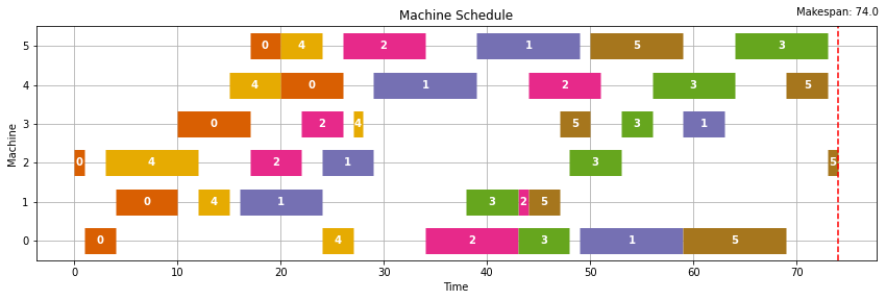
\includegraphics[width=0.8\textwidth]{Figure/gant1.png}
    \caption{Diagrama de Gantt para el cromosoma $c = [(0, 1), (16, 2), (17, 3), (38, 4), (3, 5), (44, 6)]$}
    \label{fig:gant1}
\end{figure}

\begin{table}[H]
    \centering
    \begin{tabular}{|c|c|c|c|c|}
    \hline
Trabajo & Maquina  & Comienzo  & Duración & Final \\
\hline
1    &  2   &   0     &    1    &   1\\
1    &  0   &   1     &    3    &   4\\
1    &  1   &   4     &    6    &  10\\
1    &  3   &  10     &    7    &  17\\
1    &  5   &  17     &    3    &  20\\
1    &  4   &  20     &    6    &  26\\
\hline
2    &  1   &  16     &    8   &   24\\
2    &  2  &   24    &     5  &    29\\
2    &  4  &   29    &    10  &    39\\
2    &  5  &   39    &    10  &    49\\
2    &  0  &   49    &    10  &    59\\
2    &  3  &   59    &     4  &    63\\
\hline
3    &  2  &   17    &     5  &    22\\
3    &  3   &  22    &     4   &   26\\
3    &  5  &   26   &      8  &    34\\
3    &  0  &   34   &      9  &    43\\
3    &  1  &   43   &      1  &    44\\
3    &   4  &   44   &      7  &    51\\
\hline
4    &    1  &   38   &      5  &    43\\
4    &    0  &   43   &      5  &    48\\
4    &    2  &   48   &      5  &    53\\
4    &     3 &    53  &       3 &     56\\
4    &     4 &    56  &       8 &     64\\
4    &     5 &    64  &       9 &     73\\
\hline
5    &     2 &     3  &       9 &     12\\
5    &     1 &    12  &       3 &     15\\
5    &     4  &   15   &      5    &  20\\
5    &     5   &  20   &      4    &  24\\
5    &      0   &  24  &       3   &   27\\
5    &      3   &  27  &       1   &   28\\
\hline
6    &      1   &  44  &       3   &   47\\
6    &      3   &  47  &       3   &   50\\
6    &      5   &  50   &      9   &   59\\
6    &      0   &  59    &    10   &   69\\
6    &      4   &  69    &     4  &    73\\
6    &    2   &  73      &   1   &   74\\
\hline
    \end{tabular}
    \caption{Calendario válido}
    \label{tab:calendar}
\end{table}



\subsection{FUMDAN (A Feasible UMDAc implementation for NWJSSP)}

Se empleó una adaptación del algoritmo $UMDAc$  denominado FUMDAN (A Feasible UMDAc implementation for NWJSSP), del cual se destacan 3 modificaciones descritas a continuación:

\begin{enumerate}
    \item Los individuos iniciales no son generados de manera aleatoria utilizando una distribución normal, en su lugar, se implementó una distribución normal truncada 
    
    $TN(\mu_0,\sigma_{0}^{2},0,\textit{Max Start - Job Makespan}_j)$ acotada entre 0 y $\textit{Max Start - Job Makespan}_j)$ donde \textit{Max Start} corresponde a la suma de todas las operaciones de todos los trabajos a calendarizar (Figura \ref{fig:gant2}), ${\textit{Job Makespan}}_j$ es la suma de todas las operaciones de un trabajo $j$.
    \item Se empleo una función auxiliar llamada \textit{MAKE FEASIBLE SOLUTION} \ref{alg:feasible}, la cual dado el cromosoma intenta calendarizar el trabajo j-ésimo en su retardo asignado donde si el trabajo genera una colisión con algo ya calendarizado, este se calendarizará lo mas cercano a 0 de tal forma que se eviten colisiones. 
    \item Los individuos generados al final de cada generación no son generados de manera aleatoria utilizando una distribución normal, en su lugar, se implementó una distribución normal truncada $TN(\mu_j,\sigma_{j}^{2},0,\textit{Max Start})$ acotada entre 0 y \textit{Max Start} donde \textit{Max Start} es actualizado cada vez que se encuentre un individuo cuyo \textit{Makespan} sea menor que la variable \textit{Max Start} actual.
\end{enumerate}

\begin{figure}[H]
    \centering
    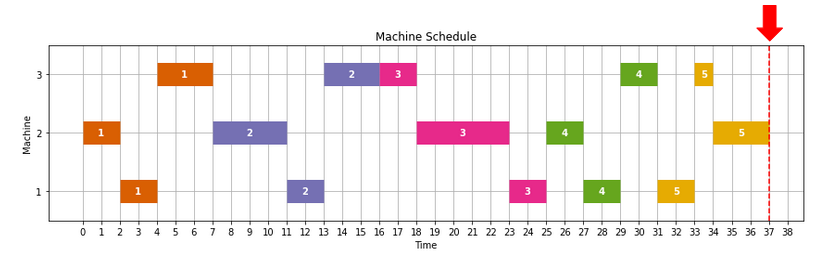
\includegraphics[width=0.8\textwidth]{Figure/max-starts.png}
    \caption{Suma de todas las operaciones de todos los trabajos para la instancia ft06, en rojo se indica el valor de $Max Start$}
    \label{fig:gant2}
\end{figure}

\begin{algorithm}[H]
\caption{FUMDAN}\label{alg:fundan}
\begin{algorithmic}[1]
\State{\textit{Max Start} $\leftarrow$ $\sum_{j\in J} o_{j\mu_{jn_j}}$} \Comment{Suma de todas las operaciones de todos los trabajos}
\State{\textit{Job }$Makespan_j$ $\leftarrow \sum o_{j\mu_{jn_j}}$ } \Comment{Suma de todas las operaciones del trabajo j-esimo}

\State{$P \leftarrow TN(\mu_0,\sigma_{0}^{2},0,\textit{Max Start - Job Makespan}_j)$} \Comment{TN Distribución Normal Truncada}
\For{generación $i = 1$ hasta $i \leq $ Generaciones }
    \For{Individuo en Población}
        \State \Call{Make Feasible Solution}{$Individuo$}
    \EndFor
    \State{Calcular $Makespan$ de cada individuo en $P$}
    \If{$Makespan$ del mejor individuo $<$ \textit{Max Start}}
    \State{\textit{Max Start} $\leftarrow Makespan$ del mejor individuo}
    \EndIf
    \State{Seleccionar $n$ individuos de $P$ utilizando \textit{Selección por torneo}}
    \State{Estimar $\mu_j$ y $\sigma_j^2$ para cada tiempo de retardo de cada Trabajo $j$}
    \State{$P \leftarrow TN(\mu_j,\sigma_j^2,0,\textit{Max Start})$} \Comment{TN Distribución Normal Truncada}
\EndFor
\end{algorithmic}
\end{algorithm}



\begin{algorithm}[H]
\captionsetup{}
\caption{MAKE FEASIBLE SOLUTION}\label{alg:feasible}
\begin{algorithmic}[1]
    \State{Ordenar el cromosoma $c = ((d_1,J_1), (d_2,J_2), \ldots (d_n,J_n))$ de acuerdo al tiempo de retardo $d_i$ con criterio de desempate $J_i$}
    \While{No se hayan calendarizado todos los trabajos}
    \State{Intentar calendarizar el trabajo $J_i$ con tiempo de retardo $d_i$ y verificar colisiones}
    \If{No existe colisiones}
        \State{Continuar con el trabajo $J_{i+1}$}
    \Else
        \State{Calendarizar $J_i$ lo mas cercano a 0}
        \State{Actualizar $d_i$ para el trabajo $J_i$}
    \EndIf
    \EndWhile
    \end{algorithmic}
\end{algorithm}
    
\section{Experimentos y Resultados}
\subsection{Configuración Experimental}
    El algoritmo propuesto fue programado utilizando el lenguaje de programación Python en su versión 3.10.4. Ejecutado en un ordenador con sistema operativo Arch Linux con kernel Linux versión 5.17.1, procesador AMD Ryzen 5 5600G @ 3.9 GHz y 16 GB de memoria RAM. El algoritmo fue evaluado en 5 instancias del ``job shop scheduling problem'' de Lawrence(1984) \cite{bksla40} y Fisher y Thompson (1963) \cite{bksft06}. Para cada instancia se realizaron 20 ejecuciones.
    
    El rendimiento del algoritmo se midió utilizando la desviación relativa porcentual (Percentage Relative Deviation, PRD) y la desviación relativa porcentual promedio (Average Percentage Relative Deviation, APRD) calculadas mediante las siguientes fórmulas:
    \begin{equation}
        PRD = {\frac{Best_{Alg} - BKS}{BKS}} \times 100\%
    \end{equation}
    \begin{equation}
        APRD = {\frac{Avg_{Alg} - BKS}{BKS}} \times 100\%
    \end{equation}
    
    Donde ${Best_{Alg}}$ es la mejor solución obtenida por el algoritmo, ${Avg_{Alg}}$ es el valor promedio de las mejores soluciones encontradas en cada una de las ejecuciones del algoritmo y $BKS$ es la mejor solución conocida de una instancia.
    
    Los parámetros utilizados para probar el algoritmo son los siguientes: tamaño de la población igual a 60, número de generaciones igual a 30, tamaño del torneo igual a 5.
    
\subsection{Resultados}
    Los resultados obtenidos se muestran en la tabla \ref{tab:my_label} donde: ``Nombre'' corresponde al nombre de la instancia, (n, m) describe el tamaño de la instancia, donde n es el número de trabajos y m es el número de máquinas, ``BK'' el valor de la mejor solución conocida para la instancia, ``avg value'' y ``std value'' el valor promedio y la desviación estandar de los valores obtenidos por el algoritmo, ``avg time'' y ``std time'' el promedio y desviación estandar del tiempo de ejecución del algoritmo, ``best'' el mejor valor encontrado por el algoritmo, ``PRD'' la desviación relativa porcentual y ``APRD'' la desviación relativa porcentual promedio.

    
    \begin{table}[H]
        \centering
        \begin{tabular}{|c|c|c|c|c|c|c|c|c|c|}
        \hline
        Nombre & (n,m) & BKS & avg value & std value & avg time & std time & best & PRD & APRD \\
        \hline
        ft06 & (6,6) & 73 & 73.45 & 1.56 & 33.76 & 3.58 & 73 & 0.00 & 0.62 \\

la05 & (10,5) & 777 & 995.40 & 20.63 & 69.42 & 3.01 & 954 & 22.78 & 28.11 \\

ft10 & (10,10) & 1607 & 1871.15 & 41.35 & 139.26 & 3.37 & 1814 & 12.88 & 16.44 \\
la40 & (15,15) & 2580 & 3719.40 & 170.14 & 417.52 & 64.77 & 3444 & 33.49 & 44.16 \\

la33 & (30,10) & 3413 & 12639.05 & 439.02 & 331.22 & 25.36 & 11733 & 243.77 & 270.32\\
\hline
        \end{tabular}
        \caption{Resultados obtenidos por el algoritmo}
        \label{tab:my_label}
    \end{table}

\section{Conclusión}

El algoritmo parece funcionar en instancias pequeñas como se pudo observar al probarlo en la instancia ``ft06'' de tamaño $ 6 \times 6$, donde además se pudo observar que requirió un tamaño de población pequeño y a su vez pocas generaciones, lo cual se traduce a pocas llamadas de la función de evaluación de aptitud. Sin embargo en problemas medianos y grandes los resultados obtenidos no fueron los esperados, obteniendo valores de \textit{PRD} entre 12\% y 33\% para problemas medianos, e inclusive llegando a valores por encima de los 240\% en instancias grandes, lo cual se traduce que el algoritmo obtuvo resultados significativamente lejanos a la mejor solución conocida. 


\newpage
\bibliographystyle{IEEEtran}
\bibliography{referencias}
\end{document}